% Options for packages loaded elsewhere
\PassOptionsToPackage{unicode}{hyperref}
\PassOptionsToPackage{hyphens}{url}
\PassOptionsToPackage{dvipsnames,svgnames,x11names}{xcolor}
%
\documentclass[
  letterpaper,
  DIV=11,
  numbers=noendperiod]{scrreprt}

\usepackage{amsmath,amssymb}
\usepackage{iftex}
\ifPDFTeX
  \usepackage[T1]{fontenc}
  \usepackage[utf8]{inputenc}
  \usepackage{textcomp} % provide euro and other symbols
\else % if luatex or xetex
  \usepackage{unicode-math}
  \defaultfontfeatures{Scale=MatchLowercase}
  \defaultfontfeatures[\rmfamily]{Ligatures=TeX,Scale=1}
\fi
\usepackage{lmodern}
\ifPDFTeX\else  
    % xetex/luatex font selection
\fi
% Use upquote if available, for straight quotes in verbatim environments
\IfFileExists{upquote.sty}{\usepackage{upquote}}{}
\IfFileExists{microtype.sty}{% use microtype if available
  \usepackage[]{microtype}
  \UseMicrotypeSet[protrusion]{basicmath} % disable protrusion for tt fonts
}{}
\makeatletter
\@ifundefined{KOMAClassName}{% if non-KOMA class
  \IfFileExists{parskip.sty}{%
    \usepackage{parskip}
  }{% else
    \setlength{\parindent}{0pt}
    \setlength{\parskip}{6pt plus 2pt minus 1pt}}
}{% if KOMA class
  \KOMAoptions{parskip=half}}
\makeatother
\usepackage{xcolor}
\setlength{\emergencystretch}{3em} % prevent overfull lines
\setcounter{secnumdepth}{-\maxdimen} % remove section numbering
% Make \paragraph and \subparagraph free-standing
\ifx\paragraph\undefined\else
  \let\oldparagraph\paragraph
  \renewcommand{\paragraph}[1]{\oldparagraph{#1}\mbox{}}
\fi
\ifx\subparagraph\undefined\else
  \let\oldsubparagraph\subparagraph
  \renewcommand{\subparagraph}[1]{\oldsubparagraph{#1}\mbox{}}
\fi

\usepackage{color}
\usepackage{fancyvrb}
\newcommand{\VerbBar}{|}
\newcommand{\VERB}{\Verb[commandchars=\\\{\}]}
\DefineVerbatimEnvironment{Highlighting}{Verbatim}{commandchars=\\\{\}}
% Add ',fontsize=\small' for more characters per line
\usepackage{framed}
\definecolor{shadecolor}{RGB}{241,243,245}
\newenvironment{Shaded}{\begin{snugshade}}{\end{snugshade}}
\newcommand{\AlertTok}[1]{\textcolor[rgb]{0.68,0.00,0.00}{#1}}
\newcommand{\AnnotationTok}[1]{\textcolor[rgb]{0.37,0.37,0.37}{#1}}
\newcommand{\AttributeTok}[1]{\textcolor[rgb]{0.40,0.45,0.13}{#1}}
\newcommand{\BaseNTok}[1]{\textcolor[rgb]{0.68,0.00,0.00}{#1}}
\newcommand{\BuiltInTok}[1]{\textcolor[rgb]{0.00,0.23,0.31}{#1}}
\newcommand{\CharTok}[1]{\textcolor[rgb]{0.13,0.47,0.30}{#1}}
\newcommand{\CommentTok}[1]{\textcolor[rgb]{0.37,0.37,0.37}{#1}}
\newcommand{\CommentVarTok}[1]{\textcolor[rgb]{0.37,0.37,0.37}{\textit{#1}}}
\newcommand{\ConstantTok}[1]{\textcolor[rgb]{0.56,0.35,0.01}{#1}}
\newcommand{\ControlFlowTok}[1]{\textcolor[rgb]{0.00,0.23,0.31}{#1}}
\newcommand{\DataTypeTok}[1]{\textcolor[rgb]{0.68,0.00,0.00}{#1}}
\newcommand{\DecValTok}[1]{\textcolor[rgb]{0.68,0.00,0.00}{#1}}
\newcommand{\DocumentationTok}[1]{\textcolor[rgb]{0.37,0.37,0.37}{\textit{#1}}}
\newcommand{\ErrorTok}[1]{\textcolor[rgb]{0.68,0.00,0.00}{#1}}
\newcommand{\ExtensionTok}[1]{\textcolor[rgb]{0.00,0.23,0.31}{#1}}
\newcommand{\FloatTok}[1]{\textcolor[rgb]{0.68,0.00,0.00}{#1}}
\newcommand{\FunctionTok}[1]{\textcolor[rgb]{0.28,0.35,0.67}{#1}}
\newcommand{\ImportTok}[1]{\textcolor[rgb]{0.00,0.46,0.62}{#1}}
\newcommand{\InformationTok}[1]{\textcolor[rgb]{0.37,0.37,0.37}{#1}}
\newcommand{\KeywordTok}[1]{\textcolor[rgb]{0.00,0.23,0.31}{#1}}
\newcommand{\NormalTok}[1]{\textcolor[rgb]{0.00,0.23,0.31}{#1}}
\newcommand{\OperatorTok}[1]{\textcolor[rgb]{0.37,0.37,0.37}{#1}}
\newcommand{\OtherTok}[1]{\textcolor[rgb]{0.00,0.23,0.31}{#1}}
\newcommand{\PreprocessorTok}[1]{\textcolor[rgb]{0.68,0.00,0.00}{#1}}
\newcommand{\RegionMarkerTok}[1]{\textcolor[rgb]{0.00,0.23,0.31}{#1}}
\newcommand{\SpecialCharTok}[1]{\textcolor[rgb]{0.37,0.37,0.37}{#1}}
\newcommand{\SpecialStringTok}[1]{\textcolor[rgb]{0.13,0.47,0.30}{#1}}
\newcommand{\StringTok}[1]{\textcolor[rgb]{0.13,0.47,0.30}{#1}}
\newcommand{\VariableTok}[1]{\textcolor[rgb]{0.07,0.07,0.07}{#1}}
\newcommand{\VerbatimStringTok}[1]{\textcolor[rgb]{0.13,0.47,0.30}{#1}}
\newcommand{\WarningTok}[1]{\textcolor[rgb]{0.37,0.37,0.37}{\textit{#1}}}

\providecommand{\tightlist}{%
  \setlength{\itemsep}{0pt}\setlength{\parskip}{0pt}}\usepackage{longtable,booktabs,array}
\usepackage{calc} % for calculating minipage widths
% Correct order of tables after \paragraph or \subparagraph
\usepackage{etoolbox}
\makeatletter
\patchcmd\longtable{\par}{\if@noskipsec\mbox{}\fi\par}{}{}
\makeatother
% Allow footnotes in longtable head/foot
\IfFileExists{footnotehyper.sty}{\usepackage{footnotehyper}}{\usepackage{footnote}}
\makesavenoteenv{longtable}
\usepackage{graphicx}
\makeatletter
\def\maxwidth{\ifdim\Gin@nat@width>\linewidth\linewidth\else\Gin@nat@width\fi}
\def\maxheight{\ifdim\Gin@nat@height>\textheight\textheight\else\Gin@nat@height\fi}
\makeatother
% Scale images if necessary, so that they will not overflow the page
% margins by default, and it is still possible to overwrite the defaults
% using explicit options in \includegraphics[width, height, ...]{}
\setkeys{Gin}{width=\maxwidth,height=\maxheight,keepaspectratio}
% Set default figure placement to htbp
\makeatletter
\def\fps@figure{htbp}
\makeatother

\usepackage{booktabs}
\usepackage{longtable}
\usepackage{array}
\usepackage{multirow}
\usepackage{wrapfig}
\usepackage{float}
\usepackage{colortbl}
\usepackage{pdflscape}
\usepackage{tabu}
\usepackage{threeparttable}
\usepackage{threeparttablex}
\usepackage[normalem]{ulem}
\usepackage{makecell}
\usepackage{xcolor}
\usepackage{siunitx}

  \newcolumntype{d}{S[
    input-open-uncertainty=,
    input-close-uncertainty=,
    parse-numbers = false,
    table-align-text-pre=false,
    table-align-text-post=false
  ]}
  
\KOMAoption{captions}{tableheading}
\makeatletter
\makeatother
\makeatletter
\makeatother
\makeatletter
\@ifpackageloaded{caption}{}{\usepackage{caption}}
\AtBeginDocument{%
\ifdefined\contentsname
  \renewcommand*\contentsname{Table of contents}
\else
  \newcommand\contentsname{Table of contents}
\fi
\ifdefined\listfigurename
  \renewcommand*\listfigurename{List of Figures}
\else
  \newcommand\listfigurename{List of Figures}
\fi
\ifdefined\listtablename
  \renewcommand*\listtablename{List of Tables}
\else
  \newcommand\listtablename{List of Tables}
\fi
\ifdefined\figurename
  \renewcommand*\figurename{Figure}
\else
  \newcommand\figurename{Figure}
\fi
\ifdefined\tablename
  \renewcommand*\tablename{Table}
\else
  \newcommand\tablename{Table}
\fi
}
\@ifpackageloaded{float}{}{\usepackage{float}}
\floatstyle{ruled}
\@ifundefined{c@chapter}{\newfloat{codelisting}{h}{lop}}{\newfloat{codelisting}{h}{lop}[chapter]}
\floatname{codelisting}{Listing}
\newcommand*\listoflistings{\listof{codelisting}{List of Listings}}
\makeatother
\makeatletter
\@ifpackageloaded{caption}{}{\usepackage{caption}}
\@ifpackageloaded{subcaption}{}{\usepackage{subcaption}}
\makeatother
\makeatletter
\@ifpackageloaded{tcolorbox}{}{\usepackage[skins,breakable]{tcolorbox}}
\makeatother
\makeatletter
\@ifundefined{shadecolor}{\definecolor{shadecolor}{rgb}{.97, .97, .97}}
\makeatother
\makeatletter
\makeatother
\makeatletter
\makeatother
\makeatletter
\@ifpackageloaded{tikz}{}{\usepackage{tikz}}
\makeatother
        \newcommand*\circled[1]{\tikz[baseline=(char.base)]{
          \node[shape=circle,draw,inner sep=1pt] (char) {{\scriptsize#1}};}}  
                  
\ifLuaTeX
  \usepackage{selnolig}  % disable illegal ligatures
\fi
\IfFileExists{bookmark.sty}{\usepackage{bookmark}}{\usepackage{hyperref}}
\IfFileExists{xurl.sty}{\usepackage{xurl}}{} % add URL line breaks if available
\urlstyle{same} % disable monospaced font for URLs
\hypersetup{
  pdftitle={7 検定},
  colorlinks=true,
  linkcolor={blue},
  filecolor={Maroon},
  citecolor={Blue},
  urlcolor={Blue},
  pdfcreator={LaTeX via pandoc}}

\title{7 検定}
\author{}
\date{}

\begin{document}
\maketitle
\ifdefined\Shaded\renewenvironment{Shaded}{\begin{tcolorbox}[breakable, enhanced, boxrule=0pt, interior hidden, sharp corners, frame hidden, borderline west={3pt}{0pt}{shadecolor}]}{\end{tcolorbox}}\fi

\hypertarget{annotated-cell-1}{%
\label{annotated-cell-1}}%
\begin{Shaded}
\begin{Highlighting}[]
\FunctionTok{rm}\NormalTok{(}\AttributeTok{list=}\FunctionTok{ls}\NormalTok{()); }\FunctionTok{gc}\NormalTok{();  }\FunctionTok{gc}\NormalTok{(); }\CommentTok{\#\textless{}1\textgreater{}}
\ControlFlowTok{if}\NormalTok{ (}\SpecialCharTok{!}\FunctionTok{require}\NormalTok{(}\StringTok{"pacman"}\NormalTok{)) }\FunctionTok{install.packages}\NormalTok{(}\StringTok{"pacman"}\NormalTok{) }\CommentTok{\#\textless{}2\textgreater{}}
\NormalTok{pacman}\SpecialCharTok{::}\FunctionTok{p\_load}\NormalTok{(tidyverse, magrittr,estimatr,car,modelsummary,ggrepel,patchwork) }\CommentTok{\#\textless{}3\textgreater{}}
\end{Highlighting}
\end{Shaded}

\begin{description}
\tightlist
\item[\circled{1}]
前の作業など,rのメモリに入っているものをリセットするコマンド
\item[\circled{2}]
パッケージ管理用のパッケージである\texttt{pacman}が入っていない場合はインストール
\item[\circled{3}]
複数のパッケージを一度に呼び出す
\end{description}

\hypertarget{ux7d71ux8a08ux7684ux4eeeux8aacux691cux5b9aux306eux8003ux3048ux65b9}{%
\section{1.
統計的仮説検定の考え方}\label{ux7d71ux8a08ux7684ux4eeeux8aacux691cux5b9aux306eux8003ux3048ux65b9}}

いわゆる回帰分析では,

\[
Y = \beta_0 + \beta_1 X_1 + ...+\beta_dX_d + \epsilon
\]

と言った線形構造を仮定して,OLS(最小二乗法)という方法で
\(\beta\)の推定値\(\hat \beta\)を推定しました。この\(\beta\)
は,説明変数\(X\)が\(Y\)とどのように関わっているのかを表します。しかし,\(\hat \beta\)はサンプルを使って推定した推定値です。母集団のパラメータである\(\beta\)とは必ずしも一致するとは限りません。しかし,中心極限定理などの確率の性質を利用すると,\(\hat \beta\)がどの程度の誤差を持って推定されたのかがわかります。特に回帰分析では想定される誤差の中に0が入っているかが重要です。
\(\beta\)が0かもしれないということは,その独立変数\(X\)が\(Y\)と関係ないかもしれない,ということを意味しているからです。

\begin{figure}

\begin{minipage}[t]{0.50\linewidth}

{\centering 

\raisebox{-\height}{

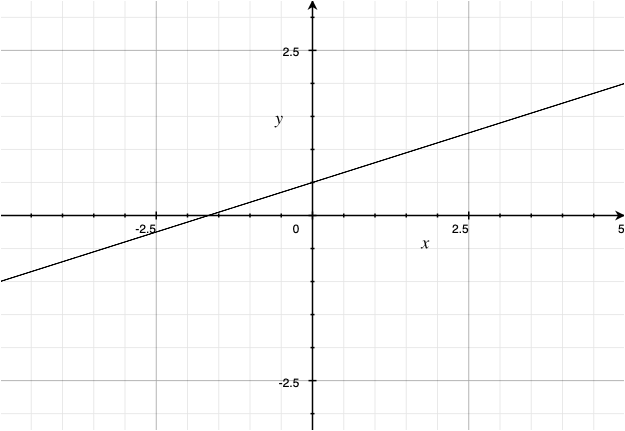
\includegraphics{images/Untitled111.png}

}

\caption{YとXに関係がある}

}

\end{minipage}%
%
\begin{minipage}[t]{0.50\linewidth}

{\centering 

\raisebox{-\height}{

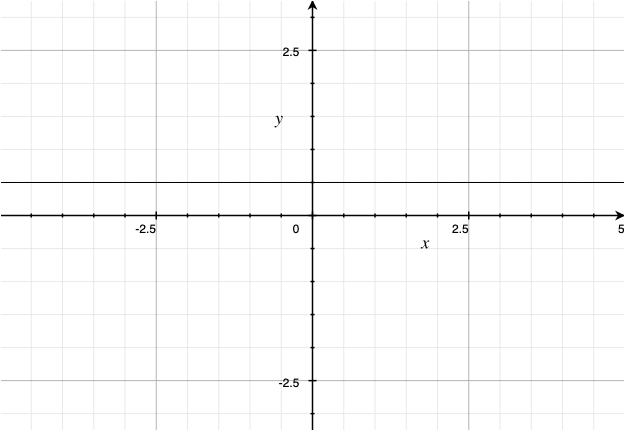
\includegraphics{images/Untitled222.png}

}

\caption{YとXに関係がない}

}

\end{minipage}%

\end{figure}

\hypertarget{ux7d71ux8a08ux7684ux4eeeux8aacux691cux5b9a}{%
\subsection{統計的仮説検定}\label{ux7d71ux8a08ux7684ux4eeeux8aacux691cux5b9a}}

このように,回帰係数に意味があるのか,についての検証は統計的仮説検定と言います。これは別に回帰分析に限ったものではなく,母集団から抽出されたサンプルを使ってなんらかの検証を行う際に広く使われます。

例えばコイントスの例です。歪みのない\footnote{高校数学でやりましたか?歪んだコインって見たことないですよね。}コインを投げた場合,表が出る確率は1/2です。今手元にあるコインが歪みのないものかどうかを検証するためには,「歪みがない」ことを仮説として持ちます。これを帰無仮説と言います。逆にこの仮説が否定されたもの「コインが歪んでいる」という仮説を対立仮説と言います。

これらの仮説を以下のプロセスで検討します。

\begin{enumerate}
\def\labelenumi{\arabic{enumi}.}
\tightlist
\item
  どれぐらいの確率なら仮説を否定するか,という基準を先に決めておく。この基準を有意水準という。
\item
  母集団の確率分布について,帰無仮説を立てる
\item
  母集団からサンプルを取得する
\item
  母集団から抽出したサンプルが母集団から得られる確率を計算し,1で決めた有意水準と比較する。優位水準より低い確率だった場合,帰無仮説が真実ではなかったとして棄却する。有意水準より大きかった場合,仮説を受容する。
\end{enumerate}

\hypertarget{ux30b3ux30a4ux30f3ux6295ux3052ux306eux30b7ux30dfux30e5ux30ecux30fcux30b7ux30e7ux30f3}{%
\subsection{コイン投げのシミュレーション}\label{ux30b3ux30a4ux30f3ux6295ux3052ux306eux30b7ux30dfux30e5ux30ecux30fcux30b7ux30e7ux30f3}}

\begin{enumerate}
\def\labelenumi{\arabic{enumi}.}
\tightlist
\item
  有意水準は(経済学や経営学では)5%や10%あたりが用いられます。5%としてみます。
\item
  帰無仮説を設定する。コインを投げて表になる確率を\(p\)
  とすると,帰無仮説\(H_0\)は \(p = \frac{1}{2}\),対立仮説\(H_1\)は
  \(p \ne \frac{1}{2}\)と設定。
\item
  コインを100回投げる。結果が表65,裏35だとする
\item
  帰無仮説が正しいとして,100回中おもてが60-40回に収まる確率を計算してみる
\end{enumerate}

\hypertarget{annotated-cell-2}{%
\label{annotated-cell-2}}%
\begin{Shaded}
\begin{Highlighting}[]
\NormalTok{p40 }\OtherTok{\textless{}{-}} \FunctionTok{pbinom}\NormalTok{(}\AttributeTok{q =} \DecValTok{40}\NormalTok{, }\AttributeTok{size =} \DecValTok{100}\NormalTok{, }\AttributeTok{prob =} \FloatTok{0.5}\NormalTok{) }\hspace*{\fill}\NormalTok{\circled{1}}
\NormalTok{p60 }\OtherTok{\textless{}{-}} \FunctionTok{pbinom}\NormalTok{(}\AttributeTok{q =} \DecValTok{60}\NormalTok{, }\AttributeTok{size =} \DecValTok{100}\NormalTok{, }\AttributeTok{prob =} \FloatTok{0.5}\NormalTok{) }\hspace*{\fill}\NormalTok{\circled{2}}
\NormalTok{p60}\SpecialCharTok{{-}}\NormalTok{p40}
\end{Highlighting}
\end{Shaded}

\begin{description}
\tightlist
\item[\circled{1}]
表が40回以下の確率
\item[\circled{2}]
表が60回以下の確率
\end{description}

\begin{verbatim}
[1] 0.9539559
\end{verbatim}

この0.9539は,コインを100回投げて,60回から40回表が出る確率を表しています。95%以上の確率で60-40会表が出る,逆に65回は5%以下と解釈できます。事前に設定された有意水準5%を下回るので,帰無仮説は棄却され,対立仮説である\(H_1\)の\(p \ne \frac{1}{2}\)が採択されます。

\hypertarget{ux56deux5e30ux5206ux6790ux3068ux7d71ux8a08ux7684ux4eeeux8aacux691cux5b9a}{%
\subsection{回帰分析と統計的仮説検定}\label{ux56deux5e30ux5206ux6790ux3068ux7d71ux8a08ux7684ux4eeeux8aacux691cux5b9a}}

\begin{itemize}
\tightlist
\item
  回帰分析についても同じ考え方で検定をします。
\item
  一般的には,説明変数が従属変数と関係ない,つまり係数\(\beta = 0\)
  を帰無仮説として検定します。
\end{itemize}

\hypertarget{ux5e73ux5747ux5024ux306eux691cux5b9a}{%
\section{平均値の検定}\label{ux5e73ux5747ux5024ux306eux691cux5b9a}}

回帰係数の検定は,平均値の検定の拡張といえます。

特に回帰分析では,\(H_0 : \mu = 0\)を検定します。

\hypertarget{ux6b63ux898fux5206ux5e03nmu1ux306eux5834ux5408}{%
\subsection{\texorpdfstring{正規分布\(N(\mu,1)\)の場合}{正規分布N(\textbackslash mu,1)の場合}}\label{ux6b63ux898fux5206ux5e03nmu1ux306eux5834ux5408}}

母集団の分布が平均\(\mu\)標準偏差1と判明しているケース

\begin{enumerate}
\def\labelenumi{\arabic{enumi}.}
\tightlist
\item
  有意水準は,5%とします。
\item
  帰無仮説\(H_0 : \mu = 0\)とすると対立仮説\(H_1 : \mu \ne 0\)となります。
\item
  検定の対象の母集団から標本を抽出します。これは大きいほうが望ましいです。ここから平均値を計算します。
\item
  もし帰無仮説が正しいのであれば,母集団は\(N(0,1)\)つまり標準正規分布であるはずです。標準正規分布に従う確率変数について,\(|X|>1.96\)となる確率が(有意水準である)5%であることが知られています。つまり,平均値の絶対値が1.96より小さかったら帰無仮説を採択,大きかったら帰無仮説を棄却して,対立仮説をとる,ということです。
\end{enumerate}

\hypertarget{tux691cux5b9a}{%
\subsection{t検定}\label{tux691cux5b9a}}

母集団の分布があらかじめわかっているということは基本的にはありません。しかし,母集団の分布がわからないという条件でも上のような検定が行える場合があります。

\begin{enumerate}
\def\labelenumi{\arabic{enumi}.}
\item
  有意水準は,5%とします。
\item
  帰無仮説\(H_0 : \mu = 0\)とすると対立仮説\(H_1 : \mu \ne 0\)となります。
\item
  検定の対象の母集団から大きさnの標本を抽出します。もし,nが十分に大きいと,中心極限定理によって,以下の\(Z_n\)は近似的に標準正規分布\(N(0,1)\)に従います。

  \[
  Z_n = \frac{\sqrt{n}(\bar{X_n} - \mu)}{\sqrt{V_n}}
  \]

  ただし,\(\bar{X_n}\)は標本平均,\(V_n\)は標本分散です。
\item
  もし帰無仮説が正しいのであれば,\(\mu = 0\)なので,\(Z_n\)は

  \[
  t_n = \frac{\sqrt{n}\bar{X_n}}{\sqrt{V_n}}
  \]

  と書き換えることができて,これが標準正規分布\(N(0,1)\)に従います。

  標準正規分布に従う確率変数について,\(|X|>1.96\)となる確率が(有意水準である)5%であることが知られています。つまり,平均値の絶対値が1.96より小さかったら帰無仮説を採択,大きかったら帰無仮説を棄却して,対立仮説をとる,ということです。
\end{enumerate}

上記\(t_n\)をt値,これを用いた検定をt検定と言います。

\hypertarget{pux5024}{%
\subsection{p値}\label{pux5024}}

上のt検定ではあらかじめ5%とか有意水準を決めていました。しかし,t値に対応させる形で,tの値がある数の時,その数字で帰無仮説を棄却するには有意水準をどこまで大きくする必要があるのか,という確率を直接求めることもできます。それをp値と言います。

t検定において,t値を見るのと,p値を見るのは本質的には同義です。p値5%がt値1.96を表しています。

\hypertarget{ux5272ux5408ux306eux691cux5b9a}{%
\chapter{割合の検定}\label{ux5272ux5408ux306eux691cux5b9a}}

\hypertarget{ux76f8ux95a2ux306eux691cux5b9a}{%
\chapter{相関の検定}\label{ux76f8ux95a2ux306eux691cux5b9a}}

\begin{Shaded}
\begin{Highlighting}[]
\NormalTok{ice3\_1 }\OtherTok{\textless{}{-}} \FunctionTok{read\_csv}\NormalTok{(}\StringTok{"data/ice3\_1.csv"}\NormalTok{)}
\FunctionTok{cor.test}\NormalTok{(ice3\_1}\SpecialCharTok{$}\NormalTok{age, ice3\_1}\SpecialCharTok{$}\NormalTok{raiten)}
\end{Highlighting}
\end{Shaded}

\begin{verbatim}

    Pearson's product-moment correlation

data:  ice3_1$age and ice3_1$raiten
t = 1.1732, df = 18, p-value = 0.256
alternative hypothesis: true correlation is not equal to 0
95 percent confidence interval:
 -0.1995311  0.6342401
sample estimates:
      cor 
0.2665227 
\end{verbatim}

\begin{Shaded}
\begin{Highlighting}[]
\NormalTok{ice3\_1 }\SpecialCharTok{\%$\%}
  \FunctionTok{cor.test}\NormalTok{(age,raiten)}
\end{Highlighting}
\end{Shaded}

\begin{verbatim}

    Pearson's product-moment correlation

data:  age and raiten
t = 1.1732, df = 18, p-value = 0.256
alternative hypothesis: true correlation is not equal to 0
95 percent confidence interval:
 -0.1995311  0.6342401
sample estimates:
      cor 
0.2665227 
\end{verbatim}

 この結果の一番下に,相関係数(`0.2665227`)が書かれています。また,
`p-value = 0.256`が検定の結果算出された有意確率です。約26\%
\textgreater{} 5\% なので,有意ではないです。

\hypertarget{ux7df4ux7fd2ux554fux984c}{%
\section{練習問題}\label{ux7df4ux7fd2ux554fux984c}}

\hypertarget{annotated-cell-5}{%
\label{annotated-cell-5}}%
\begin{Shaded}
\begin{Highlighting}[]
\FunctionTok{rm}\NormalTok{(}\AttributeTok{list=}\FunctionTok{ls}\NormalTok{()); }\FunctionTok{gc}\NormalTok{();  }\FunctionTok{gc}\NormalTok{(); }\hspace*{\fill}\NormalTok{\circled{1}}
\ControlFlowTok{if}\NormalTok{ (}\SpecialCharTok{!}\FunctionTok{require}\NormalTok{(}\StringTok{"pacman"}\NormalTok{)) }\FunctionTok{install.packages}\NormalTok{(}\StringTok{"pacman"}\NormalTok{) }\hspace*{\fill}\NormalTok{\circled{2}}
\NormalTok{pacman}\SpecialCharTok{::}\FunctionTok{p\_load}\NormalTok{(tidyverse, magrittr, modelsummary, broom) }\hspace*{\fill}\NormalTok{\circled{3}}
\end{Highlighting}
\end{Shaded}

\begin{description}
\tightlist
\item[\circled{1}]
前の作業など,rのメモリに入っているものをリセットするコマンド
\item[\circled{2}]
パッケージ管理用のパッケージである\texttt{pacman}が入っていない場合はインストール
\item[\circled{3}]
必要なパッケージを読み込み
\end{description}

\hypertarget{section}{%
\subsection{5.1}\label{section}}

\hypertarget{section-1}{%
\subsubsection{1.}\label{section-1}}

\begin{Shaded}
\begin{Highlighting}[]
\NormalTok{icecream }\SpecialCharTok{\%$\%}
  \FunctionTok{lm}\NormalTok{(icecream }\SpecialCharTok{\textasciitilde{}}\NormalTok{ income }\SpecialCharTok{+}\NormalTok{ u15) }\SpecialCharTok{\%\textgreater{}\%} 
  \FunctionTok{summary}\NormalTok{()}
\end{Highlighting}
\end{Shaded}

\begin{verbatim}

Call:
lm(formula = icecream ~ income + u15)

Residuals:
    Min      1Q  Median      3Q     Max 
-1665.6  -478.8  -118.6   613.2  2039.1 

Coefficients:
              Estimate Std. Error t value Pr(>|t|)   
(Intercept)  7.223e+03  2.114e+03   3.417  0.00134 **
income       6.424e-04  2.830e-04   2.270  0.02795 * 
u15         -8.795e+03  1.476e+04  -0.596  0.55403   
---
Signif. codes:  0 '***' 0.001 '**' 0.01 '*' 0.05 '.' 0.1 ' ' 1

Residual standard error: 871.7 on 46 degrees of freedom
Multiple R-squared:  0.1039,    Adjusted R-squared:  0.0649 
F-statistic: 2.666 on 2 and 46 DF,  p-value: 0.08028
\end{verbatim}

\hypertarget{section-2}{%
\subsubsection{2.}\label{section-2}}

\begin{Shaded}
\begin{Highlighting}[]
\NormalTok{result1 }\OtherTok{\textless{}{-}}\NormalTok{ icecream }\SpecialCharTok{\%$\%}
  \FunctionTok{lm}\NormalTok{(icecream }\SpecialCharTok{\textasciitilde{}}\NormalTok{ income }\SpecialCharTok{+}\NormalTok{ u15)}

\FunctionTok{msummary}\NormalTok{(result1,}
         \AttributeTok{statistic =} \StringTok{" [\{conf.low\}, \{conf.high\}]"}\NormalTok{)}
\end{Highlighting}
\end{Shaded}

\begin{table}
\centering
\begin{tabular}[t]{lc}
\toprule
  & (1)\\
\midrule
(Intercept) & \num{7222.763}\\
 & {}[\num{2967.362}, \num{11478.165}]\\
income & \num{0.001}\\
 & {}[\num{0.000}, \num{0.001}]\\
u15 & \num{-8795.471}\\
 & {}[\num{-38495.860}, \num{20904.918}]\\
\midrule
Num.Obs. & \num{49}\\
R2 & \num{0.104}\\
R2 Adj. & \num{0.065}\\
AIC & \num{807.5}\\
BIC & \num{815.0}\\
Log.Lik. & \num{-399.730}\\
F & \num{2.666}\\
RMSE & \num{844.57}\\
\bottomrule
\end{tabular}
\end{table}

\hypertarget{section-3}{%
\subsection{5.2}\label{section-3}}

\begin{Shaded}
\begin{Highlighting}[]
\NormalTok{tem\_aug }\OtherTok{\textless{}{-}} \FunctionTok{read\_csv}\NormalTok{(}\StringTok{"data/R\_EmpiricalAnalysis\_csv/chap04/temperature\_aug.csv"}\NormalTok{)}
\NormalTok{tem\_aug}
\end{Highlighting}
\end{Shaded}

\begin{verbatim}
# A tibble: 744 x 5
   date      time  elec  prec  temp
   <chr>    <dbl> <dbl> <dbl> <dbl>
 1 2014/8/1     0  3193     0  27.9
 2 2014/8/1     1  2960     0  27.9
 3 2014/8/1     2  2807     0  27.1
 4 2014/8/1     3  2748     0  26.8
 5 2014/8/1     4  2735     0  26.9
 6 2014/8/1     5  2736     0  27.3
 7 2014/8/1     6  2950     0  28.3
 8 2014/8/1     7  3336     0  29.4
 9 2014/8/1     8  3863     0  30.2
10 2014/8/1     9  4328     0  32.2
# i 734 more rows
\end{verbatim}

\begin{Shaded}
\begin{Highlighting}[]
\NormalTok{tem\_aug }\SpecialCharTok{\%\textless{}\textgreater{}\%}
  \FunctionTok{mutate}\NormalTok{(}\AttributeTok{morning =} \DecValTok{1}\SpecialCharTok{*}\NormalTok{ (}\DecValTok{6} \SpecialCharTok{\textless{}=}\NormalTok{ time }\SpecialCharTok{\&}\NormalTok{ time }\SpecialCharTok{\textless{}=}\DecValTok{12}\NormalTok{ ),}
         \AttributeTok{afternoon =} \DecValTok{1} \SpecialCharTok{*}\NormalTok{ (}\DecValTok{13} \SpecialCharTok{\textless{}=}\NormalTok{ time }\SpecialCharTok{\&}\NormalTok{ time }\SpecialCharTok{\textless{}=}\DecValTok{18}\NormalTok{ ))}
\NormalTok{tem\_aug}
\end{Highlighting}
\end{Shaded}

\begin{verbatim}
# A tibble: 744 x 7
   date      time  elec  prec  temp morning afternoon
   <chr>    <dbl> <dbl> <dbl> <dbl>   <dbl>     <dbl>
 1 2014/8/1     0  3193     0  27.9       0         0
 2 2014/8/1     1  2960     0  27.9       0         0
 3 2014/8/1     2  2807     0  27.1       0         0
 4 2014/8/1     3  2748     0  26.8       0         0
 5 2014/8/1     4  2735     0  26.9       0         0
 6 2014/8/1     5  2736     0  27.3       0         0
 7 2014/8/1     6  2950     0  28.3       1         0
 8 2014/8/1     7  3336     0  29.4       1         0
 9 2014/8/1     8  3863     0  30.2       1         0
10 2014/8/1     9  4328     0  32.2       1         0
# i 734 more rows
\end{verbatim}

\begin{Shaded}
\begin{Highlighting}[]
\NormalTok{tem\_aug }\SpecialCharTok{\%\textless{}\textgreater{}\%}
  \FunctionTok{mutate}\NormalTok{(}\AttributeTok{date =} \FunctionTok{ymd}\NormalTok{(date),}
         \AttributeTok{dow =} \FunctionTok{wday}\NormalTok{(date,}\AttributeTok{label =} \ConstantTok{TRUE}\NormalTok{),}
         \AttributeTok{saturday =} \DecValTok{1} \SpecialCharTok{*}\NormalTok{ (dow }\SpecialCharTok{==} \StringTok{"Sat"}\NormalTok{))}

\NormalTok{tem\_aug }\SpecialCharTok{\%\textless{}\textgreater{}\%}
  \FunctionTok{mutate}\NormalTok{(}\AttributeTok{sunday =} \DecValTok{1} \SpecialCharTok{*}\NormalTok{ (dow }\SpecialCharTok{==} \StringTok{"Sun"}\NormalTok{),}
         \AttributeTok{recess =} \DecValTok{1} \SpecialCharTok{*}\NormalTok{ (}\StringTok{"2014{-}08{-}11"}\SpecialCharTok{\textless{}=}\NormalTok{date }\SpecialCharTok{\&}\StringTok{"2014{-}08{-}11"}\SpecialCharTok{\textless{}=}\NormalTok{date ))}


  
\CommentTok{\#  mutate(saturday = 1 * ((date == "2014/8/2")|}
\CommentTok{\#                         (date == "2014/8/9")|}
\CommentTok{\#                         (date == "2014/8/16")|}
\CommentTok{\#                         (date == "2014/8/23")|}
\CommentTok{\#                         (date == "2014/8/30")}
\CommentTok{\#  ))}
\end{Highlighting}
\end{Shaded}

\begin{Shaded}
\begin{Highlighting}[]
\NormalTok{reg4\_1 }\OtherTok{\textless{}{-}}\NormalTok{tem\_aug }\SpecialCharTok{\%$\%}
  \FunctionTok{lm}\NormalTok{(elec }\SpecialCharTok{\textasciitilde{}}\NormalTok{ temp }\SpecialCharTok{+}\NormalTok{ prec }\SpecialCharTok{+}\NormalTok{ sunday }\SpecialCharTok{+}\NormalTok{ recess }\SpecialCharTok{+}\NormalTok{ morning }\SpecialCharTok{+}\NormalTok{ afternoon }\SpecialCharTok{+}\NormalTok{ saturday)}
\FunctionTok{summary}\NormalTok{(reg4\_1)}
\end{Highlighting}
\end{Shaded}

\begin{verbatim}

Call:
lm(formula = elec ~ temp + prec + sunday + recess + morning + 
    afternoon + saturday)

Residuals:
     Min       1Q   Median       3Q      Max 
-1030.02  -347.04    30.51   319.40  1012.10 

Coefficients:
            Estimate Std. Error t value Pr(>|t|)    
(Intercept)  244.956    153.145   1.600 0.110138    
temp         113.321      5.176  21.895  < 2e-16 ***
prec          14.677     16.730   0.877 0.380621    
sunday      -409.299     43.531  -9.402  < 2e-16 ***
recess      -127.016     36.236  -3.505 0.000484 ***
morning      215.088     38.074   5.649 2.30e-08 ***
afternoon    589.475     40.687  14.488  < 2e-16 ***
saturday    -260.407     43.640  -5.967 3.75e-09 ***
---
Signif. codes:  0 '***' 0.001 '**' 0.01 '*' 0.05 '.' 0.1 ' ' 1

Residual standard error: 419.8 on 736 degrees of freedom
Multiple R-squared:  0.6579,    Adjusted R-squared:  0.6547 
F-statistic: 202.2 on 7 and 736 DF,  p-value: < 2.2e-16
\end{verbatim}

\begin{Shaded}
\begin{Highlighting}[]
\FunctionTok{msummary}\NormalTok{(reg4\_1,}
         \AttributeTok{statistic =} \StringTok{" [\{conf.low\}, \{conf.high\}]"}\NormalTok{)}
\end{Highlighting}
\end{Shaded}

\begin{table}
\centering
\begin{tabular}[t]{lc}
\toprule
  & (1)\\
\midrule
(Intercept) & \num{244.956}\\
 & {}[\num{-55.697}, \num{545.609}]\\
temp & \num{113.321}\\
 & {}[\num{103.160}, \num{123.482}]\\
prec & \num{14.677}\\
 & {}[\num{-18.168}, \num{47.522}]\\
sunday & \num{-409.299}\\
 & {}[\num{-494.759}, \num{-323.839}]\\
recess & \num{-127.016}\\
 & {}[\num{-198.154}, \num{-55.879}]\\
morning & \num{215.088}\\
 & {}[\num{140.342}, \num{289.835}]\\
afternoon & \num{589.475}\\
 & {}[\num{509.598}, \num{669.351}]\\
saturday & \num{-260.407}\\
 & {}[\num{-346.080}, \num{-174.733}]\\
\midrule
Num.Obs. & \num{744}\\
R2 & \num{0.658}\\
R2 Adj. & \num{0.655}\\
AIC & \num{11108.4}\\
BIC & \num{11149.9}\\
Log.Lik. & \num{-5545.210}\\
F & \num{202.244}\\
RMSE & \num{417.51}\\
\bottomrule
\end{tabular}
\end{table}

\hypertarget{section-4}{%
\subsection{5.3}\label{section-4}}

\begin{Shaded}
\begin{Highlighting}[]
\NormalTok{S }\OtherTok{\textless{}{-}} \DecValTok{10000}
\NormalTok{box }\OtherTok{\textless{}{-}} \FunctionTok{numeric}\NormalTok{(S)}


\ControlFlowTok{for}\NormalTok{(i }\ControlFlowTok{in} \DecValTok{1}\SpecialCharTok{:}\NormalTok{S)\{}
\NormalTok{  x }\OtherTok{\textless{}{-}} \FunctionTok{rnorm}\NormalTok{(}\DecValTok{1000}\NormalTok{,}\DecValTok{0}\NormalTok{,}\DecValTok{1}\NormalTok{)}
\NormalTok{  y }\OtherTok{\textless{}{-}} \DecValTok{1}\SpecialCharTok{+}\DecValTok{5}\SpecialCharTok{*}\NormalTok{x}\SpecialCharTok{+}\FunctionTok{rnorm}\NormalTok{(}\DecValTok{1000}\NormalTok{,}\DecValTok{0}\NormalTok{,}\DecValTok{1}\NormalTok{)}
\NormalTok{  res }\OtherTok{\textless{}{-}} \FunctionTok{lm}\NormalTok{(y}\SpecialCharTok{\textasciitilde{}}\NormalTok{x) }\SpecialCharTok{\%\textgreater{}\%} \FunctionTok{summary}\NormalTok{() }\SpecialCharTok{\%\textgreater{}\%} \FunctionTok{tidy}\NormalTok{()}
\NormalTok{  beta1 }\OtherTok{\textless{}{-}}\NormalTok{ res}\SpecialCharTok{$}\NormalTok{estimate[}\DecValTok{2}\NormalTok{]}
\NormalTok{  sigma1 }\OtherTok{\textless{}{-}}\NormalTok{res}\SpecialCharTok{$}\NormalTok{std.error[}\DecValTok{2}\NormalTok{]}
\NormalTok{  box[i] }\OtherTok{\textless{}{-}}\NormalTok{ (}\FunctionTok{abs}\NormalTok{(beta1 }\SpecialCharTok{{-}}\DecValTok{5}\NormalTok{) }\SpecialCharTok{\textless{}} \FloatTok{1.96} \SpecialCharTok{*}\NormalTok{ sigma1)}
\NormalTok{\}}
\FunctionTok{mean}\NormalTok{(box)}
\end{Highlighting}
\end{Shaded}

\begin{verbatim}
[1] 0.9495
\end{verbatim}



\end{document}
